\section{Method}
\label{sec:method}

\subsection{Models and Connectors}
\label{sec:models}

We evaluate token pruning across six VLA architectures spanning three connector families (Table~\ref{tab:model_properties}; Figure~\ref{fig:architecture}). To preview each connector's compressibility, we report the coefficient of variation (CV) of post-connector token L2 norms, the ratio of standard deviation to mean across all vision tokens from a single forward pass (formally defined in Section~\ref{sec:cv_diagnostic}). \textbf{Linear projection} applies a per-patch matrix multiplication ($\pi_{0}$~\cite{black2024pi0}, $\pi_{0.5}$~\cite{black2025pi05}; CV$\,{<}\,$0.06). \textbf{MLP projectors} map each patch independently through a multi-layer perceptron (OpenVLA~\cite{kim2024openvla}, OFT~\cite{kim2025openoft}; CV$\,{\approx}\,$0.22). \textbf{Token-entangling connectors} create cross-token dependencies: X-VLA~\cite{zheng2025xvla} uses a 12-layer BART encoder~\cite{lewis2020bart} (CV$\,{=}\,$0.151); SmolVLA~\cite{shukor2025smolvla} applies pixel-shuffle $4{\times}4$ folding, concatenating 16 patches per token (CV$\,{=}\,$0.314). We classify coupling as \emph{independent} (one patch per output) or \emph{entangling} (multiple patches). Four models are evaluated in closed-loop on LIBERO~\cite{liu2023libero}; $\pi_{0}$ and OFT contribute to the CV diagnostic only.

\begin{figure*}[t]
\centering
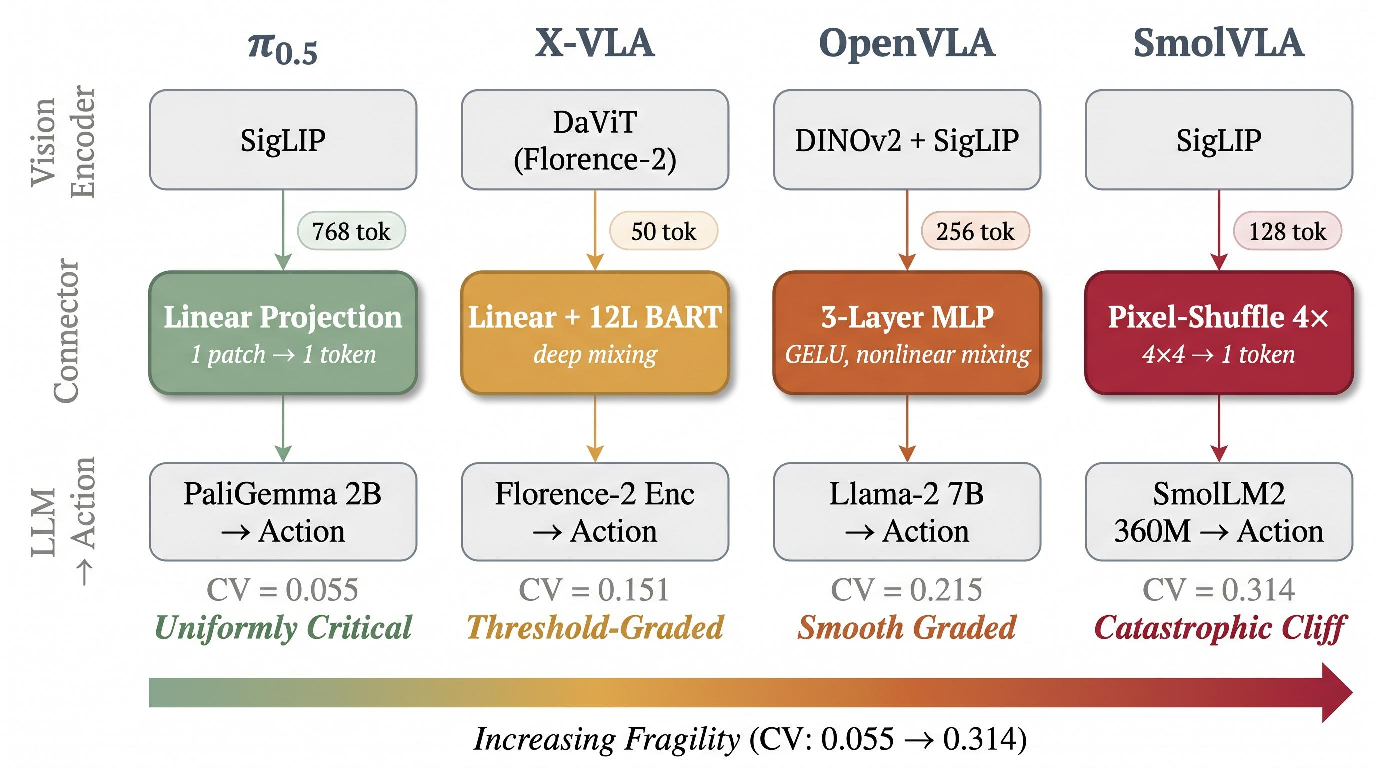
\includegraphics[width=\textwidth]{figures/paper/fig_architecture_v4.pdf}
\caption{Vision connector architectures across four closed-loop VLAs, ordered by increasing compressibility fragility. Independent connectors yield low CV; entangling connectors create cross-token dependencies and higher CV.}
\label{fig:architecture}
\end{figure*}

\subsection{Pruning Protocol}
\label{sec:pruning_protocol}

Given $N$ post-connector tokens $\{t_1, \ldots, t_N\}$ with $t_i \in \mathbb{R}^d$, token pruning retains $\lfloor k \cdot N \rfloor$ tokens for $k \in (0, 1]$ and physically removes the rest. Crucially, we \emph{re-index} the remaining positions contiguously (i.e., the $j$-th retained token receives position ID $j$) rather than preserving original position IDs. This choice isolates two confounded effects: information loss from removing tokens and position disruption from re-indexing. We prune between the connector output and LLM input to isolate the connector's effect on token information structure; the vision encoder and LLM weights remain frozen throughout.

\paragraph{Importance scoring functions.}
A scoring function $s\colon \mathbb{R}^d \to \mathbb{R}$ assigns each token an importance score; the top-$\lfloor kN \rfloor$ tokens by score are retained. We evaluate two backbone-agnostic strategies that require only the connector output, not LLM internals.

\textbf{L2-norm scoring} uses activation magnitude $s_{\text{L2}}(t_i) = \|t_i\|_2$ as a proxy for information density. For each image, we compute the L2 norm of every post-connector token, rank tokens in descending order, and retain the top-$\lfloor kN \rfloor$. L2 scoring introduces spatial bias: nearby patches share similar visual content and produce correlated norms, so aggressive pruning can concentrate retained tokens in a single spatial region at the expense of scene coverage (Section~\ref{sec:cv_sensitivity}).

\textbf{Random subsampling} draws $\lfloor kN \rfloor$ tokens uniformly without replacement ($s_{\text{rand}}(t_i) \sim \mathcal{U}(0, 1)$), providing a null hypothesis that all tokens are interchangeable. Random selection preserves spatial coverage in expectation, making it the natural baseline for spatially uniform architectures. To control sampling variance, we report results over multiple seeds (Section~\ref{sec:exp_setup}).

We also evaluate \textbf{attention-based scoring} on selected conditions: for each vision token, we sum the attention weights it receives from all action-query tokens across all LLM layers, yielding an importance score that reflects the LLM's actual usage pattern. Results appear in Appendix~\ref{app:attention_scoring}; we focus on L2 and random in the main text because they operate solely on the connector output and suffice to reveal connector-dependent importance structure.

The \emph{importance margin} $\Delta(k) = \text{SR}_{\text{L2}}(k) - \text{SR}_{\text{Random}}(k)$ quantifies exploitable importance structure at each retention ratio. A positive margin means the token importance landscape is informative: L2 norm successfully identifies dispensable tokens. A negative margin indicates L2 selection is actively harmful, clustering spatially correlated tokens while discarding critical spatial coverage. The sign and magnitude of $\Delta$ vary systematically with connector CV and $k$ (Section~\ref{sec:cv_sensitivity}).

\paragraph{Retention ratios and evaluation.}
We evaluate $k \in \{0.30, 0.50, 0.70, 0.75, 0.85, 0.90, 0.95\}$, spanning extreme compression to conservative trimming. For each model--suite--method--$k$ combination, we run all 50 evaluation episodes per task (10 tasks $\times$ 50 episodes $=$ 500 total) and report mean success rate (SR). Multi-seed conditions ($\pi_{0.5}$ Long: $n{=}5$ seeds; VTR: $n{=}3$) report mean $\pm$ sample standard deviation. This range identifies \emph{cliff zones}: narrow $k$ intervals where SR drops discontinuously. Different connectors cliff at different ratios: pixel-shuffle at $k{=}0.95$, BART-encoded near $k{\approx}0.85$, MLP without a sharp cliff (Appendix~\ref{app:pruning_details}).

\begin{table}[t]
\centering
\small
\caption{VLA models evaluated. Coupling indicates independent vs.\ cross-token processing. $N$ = vision tokens input to the LLM. $^\dagger$OFT is an OpenVLA fine-tuning variant, included for CV calibration (offline metrics only).}
\label{tab:model_properties}
\begin{tabular}{lrlcrll}
\toprule
Model & Params & Connector & $N$ & CV & Coupling & Eval \\
\midrule
$\pi_{0.5}$ & 4B & Linear ($\times\!\sqrt{d}$) & 768 & 0.055 & Indep.\ & Closed-loop \\
X-VLA & 0.9B & Linear + BART & 50 & 0.151 & Entangling & Closed-loop \\
OpenVLA & 7B & 3-layer MLP & 256 & 0.215 & Indep.\ & Closed-loop \\
SmolVLA & 450M & Pixel-shuffle $4{\times}4$ & 128 & 0.314 & Entangling & Closed-loop \\
\midrule
$\pi_{0}$ & 3.3B & Linear & 256 & 0.038 & Indep.\ & Offline \\
OFT$^\dagger$ & 7B & 3-layer MLP & 512 & 0.219 & Indep.\ & Offline \\
\bottomrule
\end{tabular}
\end{table}

\subsection{Compressibility Diagnostic: Importance CV}
\label{sec:cv_diagnostic}

We seek a zero-cost diagnostic that predicts a model's pruning tolerance without running closed-loop evaluation. The coefficient of variation (CV) of post-connector token L2 norms provides this:
\begin{equation}
\text{CV} = \frac{\sigma\!\left(\{\|t_i\|_2\}_{i=1}^{N}\right)}{\mu\!\left(\{\|t_i\|_2\}_{i=1}^{N}\right)}
\label{eq:cv}
\end{equation}
where $\sigma$ and $\mu$ denote the standard deviation and mean over all $N$ post-connector tokens from a single forward pass. CV requires no labeled data, no downstream task evaluation, and no access to the LLM backbone.

\paragraph{The CV spectrum.}
CV captures a continuous ordering across six models and three connector families (Table~\ref{tab:model_properties}). Linear projections yield the lowest values ($\pi_{0}$: 0.038 (offline), $\pi_{0.5}$: 0.055), followed by X-VLA's BART encoder (0.151), the MLP projectors of OpenVLA and OFT (0.215, 0.219), and SmolVLA's pixel-shuffle at the high end (0.314). The progression reflects increasing cross-token entanglement: linear projections produce near-uniform norms (CV$\,{<}\,$0.06), MLP nonlinearities amplify variance (CV$\,{\approx}\,$0.22), and pixel-shuffle creates maximal entanglement.

\paragraph{CV as pruning tolerance predictor.}
High CV means some tokens carry substantially larger norms; these can be retained while low-norm tokens are removed with limited loss. Low CV means near-uniform norms: pruning becomes equivalent to downsampling a uniform signal, where spatial coverage matters more than importance ranking. CV also predicts the optimal scoring strategy: when CV$\,{<}\,$0.15, random outperforms L2 by preserving spatial coverage; when CV$\,{>}\,$0.20, L2 exploits genuine importance differentiation. The importance margin $\Delta$ increases monotonically with CV across three closed-loop models (Section~\ref{sec:cv_sensitivity}). Attention entropy provides a complementary but less discriminative signal (Appendix~\ref{app:attention_entropy}).

\subsection{Vision Token Re-encoder (VTR)}
\label{sec:vtr}

Hard pruning fails for token-entangling connectors because removing any token destroys spatially distributed information. VTR addresses this through learned re-encoding rather than deletion.

\paragraph{Architecture.}
VTR inserts a 2-layer cross-attention module (12 heads) between the connector output and the LLM input. $M$ learned queries attend over all $N$ source tokens, producing $M$ compressed tokens ($M \in \{16, 32, 64, 96, 128\}$). The module adds ${\sim}$22M parameters ($<$5\% of SmolVLA) and is trained end-to-end (Appendix~\ref{app:smart_compress_details}).
